\documentclass[onecolumn, draftclsnofoot,10pt, compsoc]{article}
\usepackage{graphicx}
\usepackage{url}
\usepackage{lscape}
\usepackage{setspace}
\usepackage{parskip}
\usepackage{geometry}
\usepackage{listings}
\geometry{textheight=9.5in, textwidth=7in}

% 1. Fill in these details
\def \CapstoneTeamName{AgBizClimate}
\def \CapstoneTeamNumber{26}
\def \GroupMemberOne{}%Your Name Here
\def \CapstoneProjectName{ Linking Seasonal Weather Data to AgBizClimate\texttrademark}
\def \CapstoneSponsorCompany{ Oregon State University}
\def \CapstoneSponsorPerson{ Clark Seavert}

% 2. Uncomment the appropriate line below so that the document type works
\def \DocType{		%Software Requirements Document
				%Requirements Document
				%Technology Review
				%Design Document
				Final Progress Report Winter 2018
				}

\newcommand{\NameSigPair}[1]{\par
\makebox[2.75in][r]{#1} \hfil 	\makebox[3.25in]{\makebox[2.25in]{\hrulefill} \hfill		\makebox[.75in]{\hrulefill}}
\par\vspace{-12pt} \textit{\tiny\noindent
\makebox[2.75in]{} \hfil		\makebox[3.25in]{\makebox[2.25in][r]{Signature} \hfill	\makebox[.75in][r]{Date}}}}
% 3. If the document is not to be signed, uncomment the RENEWcommand below
\renewcommand{\NameSigPair}[1]{#1}

%%%%%%%%%%%%%%%%%%%%%%%%%%%%%%%%%%%%%%%
\begin{document}
\begin{titlepage}
    \pagenumbering{gobble}
    \begin{singlespace}
        \hfill
        % 4. If you have a logo, use this includegraphics command to put it on the coversheet.
        %\includegraphics[height=4cm]{CompanyLogo}
        \par\vspace{.2in}
        \centering
        \scshape{
            \huge CS Capstone \DocType \par
            {\large\today}\par
            \vspace{.5in}
            \textbf{\Huge\CapstoneProjectName}\par
            \vfill
            {\large Prepared for}\par
            \Huge \CapstoneSponsorCompany\par
            \vspace{5pt}
            {\Large\NameSigPair{\CapstoneSponsorPerson}\par}
            {\large Prepared by }\par
            Group\CapstoneTeamNumber\par
            % 5. comment out the line below this one if you do not wish to name your team
            %\CapstoneTeamName\par
            \vspace{5pt}
            {\Large
                \NameSigPair{\GroupMemberOne}\par
            }
            \vspace{20pt}
        }
        \begin{abstract}
					%Write Abstract here.
					The purpose of this document is to give a snap shot of the current state of the \textit{AgBizClimate} project. In this progress report I will start off by giving a short introduction of the project and project goals. Then I will discuss the current state of the project. This will include resolved work items, work items in progress, completed work items and major blockers. The next section will include specific details of my contribution to the project including figures and interesting code. Next I will discuss a weekly summary of progress. This section will include plans, progress, problems and a summery for each week of work this term. Next I will provide a retrospective for development this last term. The retrospective will include a column for positive things that happened this that happened this term, things that need to change and another column for actions we will need to take to implement those changes. The last section will provide a peer review for each group member inducing a brief self review.\\
        \end{abstract}
    \end{singlespace}
\end{titlepage}
\newpage
\pagenumbering{arabic}
\tableofcontents
% 7. uncomment this (if applicable). Consider adding a page break.
%\listoffigures 
\newpage
%\listoftables
\clearpage

% 8. now you write!
%this section can likely be coppied from the design doc.
\section{Introduction}
	\subsection{Purpose}
		The purpose of this document is to describe the progress we have made so far on the \textit{AgBizClimate} project. In this document we will give a brief introduction to the \textit{AgBizCliamte} project. In this section we will discuss the purpose of the project. Additionally, we will also discuss the scope of the project and an overview of the project functions.\\
		This document is designed for the project owners. This document is also designed for the development team so we can evaluate our progress so far on this project. This project is also designed to fulfill the minimum requirements for the CS461 class for the OSU computer science program.\\

				\subsection{Overview}
			Seasonal climate is one of the essential factors that affects agricultural production. As a module of \textit{AgBiz Logic}, \textit{AgBizClimate} delivers essential information about climate change to farmers, and help professionals to develop management pathways that best fit their operations under a changing climate. This project aims to link the crucial seasonal climate data from the Northwest Climate Toolbox database to \textit{AgBiz Logic} so that it can provide changes in net returns of crop and livestock enterprises through powerful graphics and tables.\\

		\subsection{Scope}
			This project is a part of a much larger AgBiz Logic\texttrademark program. However, the purpose of this project is to add a short term climate tool to the \textit{AgBizClimate} module. This limits the scope of the project to the \textit{AgBizClimate} Module. Additionally, we will only be adding the short term climate data tool as the long term climate data tool already exists.\\

			Currently \textit{AgBizClimate} has a long-term climate tool but no such tool exists for short term climate data. We will implement a tool to extract short-term climate data from the Northwest Climate Toolbox database, display it to the user and allow the user to adjust crop and livestock yields or quality of products sold and, production inputs. Moreover, a landing tool will be developed to allow users to switch between short-term seasonal tool and long-term climate data tool.\\

		\subsection{Definitions, Acronyms and Abbreviations}
			REST - Representational State Transfer, This is a type of architecture that manages the state of the program. This is especially popular in web development.\\
			API- Application Programming Interface. This is a piece of software that allows a connection to another piece of software providing some sort of service.\\
			NWCTB - Northwest Climate Toolbox. This is the database we will be connecting to that will provide the short term climate data we plan to use.\\
			Thredds Data Server - This is a web server that provides meta-data and data access for scientific data sets using OPeNDAP along with some other remote data access protocols.\\
			OPeNDAP - Open-source Project for a Network Data Access Protocol. This is the protocol we will be using to retrieve the data sets from the Thredds data server.\\
			NMME - North American Multi-Model Ensemble. This is a data set that brings together a variety of different weather models into one data set.\\
			Climate Scenario - This is a theoretical calculation of yields, inputs and of the overall budget for one situation based on the climate data.\\
			NETCDF - This is a file storage format for large scientific data sets especially good for any data that is referenced on a grid and related to is geo-location.\\


		%will need updates.
		\subsection{Product Function Overview}
		    \textit{AgBizClimate} is a web based decision tool that will allow users to gain specific insight on how localized climate data for the next seven months will affect their crop and livestock yields or quality of products sold and production inputs. The \textit{AgBizClimate} tool will allow users to input their location (state, county) and a budget for the specific crop or livestock enterprise. \textit{AgBizClimate} will select climate data for the next seven months for that location and provide graphical data showing temperature and precipitation. Users will then be able to change yields or quality of product sold by a percentage they think these factors will affect and modify production inputs. Finally the tool will calculate the net returns.\\

\section{Current Project State}
In this section we will list the work items we have completed, the work items that are in progress and the work items that still need to be completed. For each work item we will also give a brief description.\\

	\subsection{Resolved Items}
		\subsubsection{Updated Requirements Document:}
		Earlier this term I made updates to the Requirements document to reflect the changes to our access to our data source for the short term climate data.\\
		
		\subsubsection{Created Climate Data API:}
		Over the last development period much progress has been made on the climate data API. This API now uses an HTTP request to scrape the data we need from the NMME data set from the Northwest Climate knowledge database. This API is able to reliably get data for most locations.\\
		
		\subsubsection{refined the Charts page:}
		We've also made significant improvements to the charts page that we created in the last development cycle. This page now gets dynamically generated data from the backend API. We've also fixed several bugs with this page that caused the budgets page to not be loaded.\\
		
		\subsubsection{Created end point for Climate API:}
		Along with creating the end point for the climate data API we also created an end point to serve the data created by the API. This end point takes a State and County and calculates an approximate latitude and longitude for that location. The end point then uses the latitude and longitude to get the data for that location using the climate data API mentioned above. The data is then formatted with labels and returned to the client.\\
		
		\subsubsection{Bug Fixes:}
		As mentioned previously we have made several bug fixes through out this last development cycle. Some of these bug fixes have involved the charts page. One bug prevented the application from going to the budgets page after the charts page. Another bug was introduced because of the introduction of short term climate budgets. This bug prevented the user from using multiple budgets because we could not distinguish between long term scenarios and short term scenarios. We were able to fix these bugs created by introducing new code in to the project over this last development cycle.\\
		
		\subsubsection{Front End Unit Tests:}
		Finally, We wrote front end unit tests for the code added to project along with updating existing unit tests to reflect changes made to the application. Currently all front end unit tests pass.\\
		
	\subsection{In progress}
		\subsubsection{refining climate API endpoint:}
		We are currently in the process of refining our climate API end point. We will need to move the code that actually goes out to the climate database and gets the data as currently it is in the same file as the end point. We will also need to add some error handling for some special cases that we have determined we are likely to encounter. Firstly, we will need to handle the case where a location doesn't have any climate data. Secondly, we will also need to handle the case where the climate data is being updated as this happens once a month and can take as long as three days.\\
		
		\subsubsection{Bug Fixes:}
		As is typical with most software development projects there will always be bugs to fix. As a result we have several bugs to fix in our application currently. One bug involves the deletion of a climate scenario. Sometimes deleting a climate scenario causes a 500 error. Another bug involves what we do if for some reason our data source for the short term data times out.\\
		
		\subsubsection{Front End Responsiveness Testing:}
		We also need to do some testing that ensure that the UI elements that the user clicks on produce the desired results. As part of the frame work for of the JS testing frame work we are using for this project we can do responsiveness testing. Currently, this process has been started but will need to be finished.\\

	\subsection{ToDo's}
		\subsubsection{Back End Testing:}
		The back end code we created to get the climate data will need to be tested. Additionally we will also need to test the end point that this code lives in. Specifically, we need to test that the conversion from county and state to lat long is as accurate as possible.\\
		
		\subsubsection{Document Updates:}
		We will need to update several documents including our design document, the requirements document, the technical review and our expo poster. Most of these items will need to be updated as a result of design choices we made over the term regarding the project.\\

		\subsubsection{Blockers:}
		Currently, we have no major blockers. The one major blocker we had at through out the beginning of the term we resolved when we found a better way to get the climate data from the database.\\

\section{My Contributions}
	In this section I will discuss my contributions to this project. This section will discuss specifically contributions I've made to the project along with any interesting screen shots or any interesting snipets of code.\\

		\subsection{Back End Development Using NETCDF:}
		Early in the term we tried to develop the climate data API using NETCDF over the OPENDAP protocol. In the long run we ended up abandoning this method of getting the data from the database. Never the less, early in the term I spend a decent amount of time creating a concept script that using NETCDF4, a python module, to get data from the NMME thredds server. It is unfortunate that we were unable to use this method as it would have been simpler than the method we ended up using, at least in terms of the code. Shown below is a code snipet that shows how to get a particular data point from the database using the NETCDF4 library.\\
		
\begin{lstlisting}
	#set up the data handles to filter the data
	filehandle = Dataset(path, 'r', format="netcdf3")
	lathandle = filehandle.variables['lat']
	lonhandle = filehandle.variables['lon']
	datahandle = filehandle.variables['prate_anom']

	#gets data from the server.
	print(datahandle[466, 1083, 0])
\end{lstlisting}
		
		As you can see getting data from the sever using NETCDF4 is much like using a multi-dimensional array. Essentially there are three indecencies one for latitude, one for longitude and one for time. However, we later found that though this method was easy to use that it was not particularly reliable. We ended up finding issues with reading file chucks from the remote server that we could not diagnose. I even presented this to the NETCDF4 development team through an issue on github, however they wouldn't fix it because we could not identify where in the many layers of software the problem was happening. Luckily one of my team mates found a work around so I passed on development of the API to him.\\
	
		\subsection{Front End Development:}
		For the later half of the term I ended up working on the front end of the application. This development was done using JavaScript through a frame work called Angular. Though I ended up working on many different pages and models on the front end the majority of my development efforts were focused on the charts page. The goal of the charts page is to display charts to the user so that they can make adjustments to their yields based on the data presented in the charts. Shown below is a screen shot of this page.\\
		
		%include graphic of charts page here.
		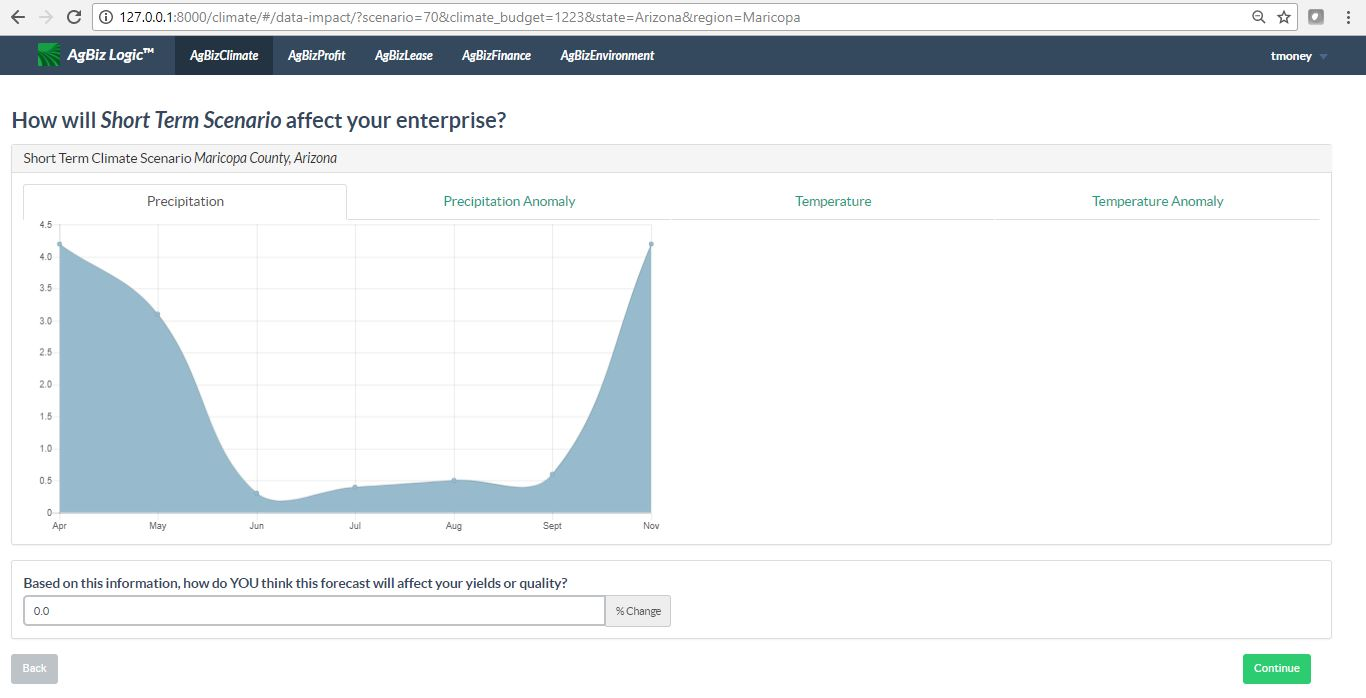
\includegraphics[width=\paperwidth,scale=0.75]{Images/ChartsPage.JPG}
		
	As you can see from the above graphic this page has four tabs which allow the user to switch between the four different charts the user can view. There is also an input box at the bottom of the page that will validate the users input ensuring that the enter a number with one decimal place.\\
	
	The majority of the challenge of building this page was not actually the UI elements. I was able to get those set up and working fairly quickly. Rather the main challenge was setting up all the budgets required for this page and the budget page following. Though this page may seem simple, there are actually many different data structures that need to be managed so that the yield on the budget is adjusted correctly, saved to the database and then passed to the budget editor after the user enters their yield. This page must also get the climate data from the back end and make sure that this data is valid.\\
	
	Another major section of front end development this term was modifying the rest of the front end to accommodate the creation of short term climate scenarios. Before we started working on this application short term climate scenarios did not exist. Thus the path through the application that is currently used for short term climate scenarios did not exist. The existing code had to be modified to allow us for branching off in to the short term climate scenario.\\
	
		\subsection{Testing:}
		Another part of the project that I worked on was Testing. In particular over this last term I've worked the front end unit tests. This involved writing test for the Charts Page that I created and updating existing tests based on changes I made to the front end of the application. I also ensured that the code I added in other parts of the application was properly tested.\\
		
		While testing one of the things I like about the testing framework we are using is that you can mock the various dependencies that any particular page may need. For instance lets say I need to make a call to the back end to update a budget. Rather than actually have to spin up the back end and call it and test that the correct action is taken, I can simply pass the front end a mock service and tell it to return a predefined value. An example of this code is shown below.\\
		
		\begin{lstlisting}
it("checks state parameters for scenario id and calls data service to retrieve scenario", 
function() {
		spyOn(climateServiceMock, "retrieveScenario").and.callThrough();
		$state.params = {'scenario': 1};
		controller.$onInit();
		$scope.$digest();

    expect(climateServiceMock.retrieveScenario.calls.argsFor(0)).toContain(1);
    expect($state.go).not.toHaveBeenCalled();
 });
		\end{lstlisting}
		Notice the spyOn function above what that does is it sates the service mock object you'd like to mock along with the specific function you are interested in. Then you can do various things. This example just skips over the function call however you can also tell the mock object to return data or to throw exceptions. What this allows you to do is test the front end code with out any other dependencies. This allows you to better trust the results of your tests.\\
		
		
		\subsection{Project Management:}
		Over the course of the term I have also spent some time managing the project. For the most part I've set all the project goals and time tables. I've also delegated tasks based on what people are interested in and what they are good at. I also set up the github repo and have been central in setting up meetings with our client. Additionally, I've been adding issues to our github repo so that we can track the progress of our project.\\
		
%will copy from one note. Will need to modify weekly summary from each week just a tiny bit to make this section work
\section{Weekly summary of progress}
	   In this section we will give a weekly summary of our progress on this project. For each we will list out our plans, problems we have encountered during the week and will show a summery of what we have accomplished during the week.\\

		\subsection{Week 1}
			\subsubsection{Plans}
				\begin{itemize}
					\item Meet with group to set up iteration one of project development.
					\item Meet with Sean to set up git branch and discuss git workflow.
					\item set tasks for iteration 1.
				\end{itemize}

			\subsubsection{Progress}
				\begin{itemize}
					\item Forked github repo from AgBiz-Logic
					\item Set up a meeting with Sean to discuss project development.
					\item Started setting up tasks for iteration one on the git repo.
					\item Started working on the Wiki page with common help items for the project.
				\end{itemize}
			\subsubsection{Problems}
				\begin{itemize}
					\item Still haven't heard any thing from the NWCTB team regarding API access for the climate data.
				\end{itemize}

			\subsubsection{Summary}
			This week we tried to set up a meeting with Sean to do some project planning and set up for iteration one of our project. However, Sean was unavailable this week so we set up a meeting for next week. We also got our git repo, forked from \textit{AgBiz-Logic} set up. We started planning the first iteration of development on the project by adding issues to the github repository. We also started compiling some help pages on the Wiki of our repo.\\

		\subsection{Week 2}
			\subsubsection{Plans}
				\begin{itemize}
					\item Meet with Sean.
					\item Start Iteration One.
					\item Get UI elements implemented along with most of the front end functionality.
					\item Plan iterations 2 and 3.
				\end{itemize}
			\subsubsection{Progress}
				\begin{itemize}
					\item Set up meeting with Sean Hammond for Friday at 1 pm.
					\item Finished setting up iteration one tasks.
					\item Finished adding content to the help wiki on the github repository.
					\item Finally defined Climate Data API Access.
					\item Set a Weekly status meeting time to meet with the group. We plan to meet every week at one pm.
				\end{itemize}
			\subsubsection{Problems}
				\begin{itemize}
					\item API Access is less than ideal and will require more work than we were planning on but is still better than having to write our own service from scratch.
					\item Finding time to meet up as a group has been more challenging that I had anticipated.
				\end{itemize}

			\subsubsection{Summary}
			This week we didn't get much development work done on our project like we had planed on. However, we did do some set up work. we finished setting up the github repository and finished laying out tasks on our story board. We also started defining what tasks we'd like to have in future iterations of our project. Additionally, we finally know what our API access to the climate data looks like. this will allow us to get the data we will need to plot. However, this will also require much more work that we had planned on and may set us back a bit in terms of our project schedule. That being said we worked in some flex time in to our schedule so we should be able to make it work.\\

		\subsection{Week 3}
			\subsubsection{Plans}
				\begin{itemize}
					\item Create proof of concept script for connecting to the database and getting data.
					\item start working on front end changes.
					\item Update design document and requirement document.
					\item Meet with Sean for status update at 1pm on Friday.
				\end{itemize}
			\subsubsection{Progress}
				\begin{itemize}
					\item Started working on concept script.
					\item Managed to gt dev environment set up instructions completed.
					\item Installed netcdf.
					\item Created example script for getting climate data from the thredds database. However we get some errors on certain reads.
					\item Updated requirements document.
				\end{itemize}
			\subsubsection{Problems}
				\begin{itemize}
					\item We had a hard time getting NETCDF4 to install. We ended up using anaconda however we are guessing Sean doesn't want to use Anaconda and will want us to produce an install script.\\
				\end{itemize}
			\subsubsection{Summary}
			This week was a primarily a week of setup. we spent most of our time trying to get the dev environment set up along with installing NETCDF4 and its dependencies. This week we did find a way to install NETCDF4 using anaconda. However, we anticipate that we will be required to find a better way to install it. In the mean time this will allow us to develop a concept script. We also managed to the development environment for AgBiz-Logic set up. This took us more time that we had anticipated but wasn't as difficult as we thought it might be. This week we also made some updates to the requirements document to reflect the changes to the climate data API.\\

		\subsection{week 4}
			\subsubsection{Plans}
				\begin{itemize}
					\item Start working on the front end of the application.
					\item Refine the proof of concept to be more dynamic.
					\item Write script to install netcdf and dependencies.
					\item Start working on backend changes.
					\item Update documents.
				\end{itemize}
			\subsubsection{Progress}
				\begin{itemize}
					\item Started working on refining proof of concept script to search for points if the point we asked for doesn't have data also added more advanced bounds checking.
					\item Determined that NETCDF4 is having issues reading in blocks for chunk three.
				\end{itemize}
			\subsubsection{Problems}
				\begin{itemize}
					\item requests past index 435 on latitude cause a runtime error.
				\end{itemize}
			\subsubsection{Summary}
			This week was mostly focused on working on the proof of concept scrip that will be used later to access the data from the thredds server. This week we discovered that the NETCDF4 library throws errors on any lat index greater than 435. We also discovered through the database administrator that this is the boundary between chunk two and chunk three of the file we are trying to read. We think that the NETCDF4 library may have a bug in it. Regardless we are going to need to find a work around moving forward. Shane and Thomas also got together on Saturday and started working on front end changes.\\

		\subsection{week 5}
			\subsubsection{Plans}
				\begin{itemize}
					\item Work on front end changes.
					\item Follow up with NETCDF4 developers about potential bug.
					\item Continue to work on concept script to see if we can tease out the runtime error.
					\item Finish NETCDF5 install script.
					\item Research other potential options other than python or netcdf4 for reading in data from the serer.\\

				\end{itemize}
			\subsubsection{Progress}
				\begin{itemize}
					\item Followed up with netcdf4 people.
					\item Shane finished the netcdf4 install script.
					\item Researched alternatives to netcdf4 We can write a c program that will to the same thing. There are a few other libraries for reading data via opendap.
					\item made progress on frontend changes.
				\end{itemize}

			\subsubsection{Problems}
				\begin{itemize}
					\item Issues with netcdf4 library.
					\item netcdf4 developers will not fix unless I can produce a self contained example of the read failing.
					\item We think that netcdf4 dependencies may not be installed correctly.
				\end{itemize}

			\subsubsection{Summary}
			 This week we made progress on the front end development and installing the dependencies for netcdf. However, we've run into some issues with netcdf. We think we maybe able to fix it by installing the dependencies for netcdf from source with certain flags enabled but we aren't totally sure on that. We also started work on setting up the end point where the API will live. The plan for now is to have it serve mock data as to enable us to continue with the rest of the development work without getting behind.\\

		%will fill out this section later this week.
		\subsection{week 6}
			\subsubsection{Plans}
				\begin{itemize}
					\item Finish development of the charts page.
					\item Set up API to mock data.
					\item Figure out work around for netCDF problems.
					\item write the midterm progress report.
					\item make the midterm progress presentation.
					\item finish the poster rough draft.
				\end{itemize}
			\subsubsection{Progress}
				\begin{itemize}
					\item Finished Development on the charts page.
					\item Finished the midterm progress report.
					\item Made the midterm progress report presentation.
					\item Finished the Poster rough draft.
					\item Found a work around for NETCDF4 issues.
				\end{itemize}
			\subsubsection{Problems}
				\begin{itemize}
					\item Created some bugs by introducing short term climate scenarios.
						\subitem There are many ways we can fix this problem we will need to discuss with Sean how he wants this solved.
				\end{itemize}
			\subsubsection{Summary} This week was a busy week. This week we accomplished most of the front end development required by this project in the maps page. However, we also introduced some bugs. Mostly we created and issue where if you have multiple budgets its not possible to tell what page you need to redirect to once you save your budget. There are many ways we can solve this so I want to ask Sean how he thinks the best way to go about this is. This week we also made our expo poster along with creating the midterm progress report document and presentation. Additionally, Shengpei found a work around to the NETCDF problems we've been having.\\
			
		\subsection{week 7}
			\subsubsection{Plans}
				\begin{itemize}
					\item Fix bug with short term climate scenario where rap around for multiple budgets doesn't work.
					\item Translate Shengpei's concept script from python 3.6 to 2.7.
					\item Create end point to host climate API.
					\item Serve static data from the end point to the front end until API is set up to get dynamic data.
					\item Integrate Shengpei's API into the end piont.
				\end{itemize}
			\subsection{Progress}
				\begin{itemize}
					\item Fixed Bug with rapping around for multiple budgets.
					\item Shengpei translated script into python 2.7.
					\item Shane worked on getting end point setup.
				\end{itemize}
			\subsection{Problems}
				\begin{itemize}
					\item Shengpei's script needs to refined.
					\item Inexperience with Django.
				\end{itemize}
			\subsubsection{Summary} This week we continued to work on the frontend of the application. We made progress on getting some of the bugs fixed on the front end. Mainly, Now when you use multiple budgets the application correctly redirects to the correct page once reaching the end of the work flow. Shengpei also managed to get his script ported over from python 3.6 to python 2.7. Shane worked on setting up the endpoint that will evenutally host the climate data API. However, we ran into a few issues with this due to inexperience with Django.\\
			
		\subsection{week 8}
			\subsubsection{Plans}
				\begin{itemize}
					\item Create Unit tests for the Data-Impact page.
					\item update existing unit test to reflect changes in the application.
					\item Get end point up and running.
					\item Refine Shengpei's script so it returns data we can consume.
				\end{itemize}
			\subsection{Progress}
				\begin{itemize}
					\item Updated existing front end tests.
					\item Started working on Unit tests for the front end.
					\item started working on changes to API to make the data consumable.
				\end{itemize}
			\subsection{Problems}
				\begin{itemize}
					\item Having issues with mocking the services on the front end correctly.
				\end{itemize}
			\subsubsection{Summary} This week we worked on setting up the back end to serve the data to the front end. We also started working on the front end unit tests. Additionally Shengpei started working on updating the API. It's looking increasingly more likely that we can have a beta next week if not early in week 10.\\
			
		\subsection{week 9}
			\subsubsection{Plans}
				\begin{itemize}
					\item Finish Front end testing.
					\item Get climate data endpoint up and running.
					\item Finish updates to the climate API.
					\item Set up front end to use endpoint to dynamically get data.
				\end{itemize}
			\subsection{Progress}
				\begin{itemize}
					\item Finished front end testing.
					\item Finished setting up end point.
					\item Finished refining the API.
				\end{itemize}
			\subsection{Problems}
				We had no major problems during this week of development.\\
			\subsubsection{Summary} This week we continued to make progress on the development of our application. I finished up the front end unit tests and they now all pass. Shane set up the end point and has it ready to consume the API. Shengpei finished making the updates to the API so that the front end can easily consume the data. All that is left to do is to put the pieces together and fix any bugs we've created in the process. Next week we should be able to put the pieces together and produce a fully functioning beta release.\\

		\subsection{week 10}
			\subsubsection{Plans}
				\begin{itemize}
					\item Create Beta Release.
					\item Start Testing and bug fix phase of the project.
					\item Write and present final progress report.
					\item Integrate API into end point to serve data.
					\item set up front end to call the end point to get the dynamically generated data.
				\end{itemize}
			\subsection{Progress}
				\begin{itemize}
					\item Shane integrated the API in to the end point so our API is now serving dynamically generated data.
					\item Set up front end to call the end point and get the dynamically generated data. With the completion of this item we now have a fully functional beta release.
					\item Created progress report template.
					\item Meet with Sean to demo beta release.
				\end{itemize}
			\subsection{Problems}
				\begin{itemize}
					\item Need to write some code to deal with when the Climate data server is under maintenance.
				\end{itemize}
			\subsection{Summary} This week we took all the pieces that we already had done and put them together. We found a few issues with the climate API and fixed them. Shane integrated the climate data end point with the climate data API. I then used that end point to get dynamically generated data on the front end. Thus we now have a fully functional beta.\\
		

\section{Retrospective}
	\begin{center}
		\begin{tabular}{| p{0.3\linewidth} | p{0.3\linewidth} | p{0.3\linewidth} |}
		\hline
		Positives & Deltas & Actions \\ 
		\hline
			We managed to Get caught Up despite being behind after the first few weeks of the term.
			& Will need to change gears to updating documents.
			& Set goals for dates we would like to have each document complete.  \\ 
		\hline
			Were much more intentional about meeting as a group to work on the project. As a result we worked much better as a team. 
			& Need to switch gears and start regression testing the application 
			& Will need to set testing goals for what we would like to have tested and when. \\ 		\hline
			We spread the work load more evenly across team members. &
			We need to be better about keeping each other updated on progress of work items &
			Have daily stand up meetings either in person or digitally. Message on slack when checking in a work item into github.\\
			\hline
				
		
		
	
	\end{tabular}
\end{center}
	
	
\section{Peer Reviews}
	In this section I will review my peers performance through out the term. I will rate their performance based on their performance as a team member along with their contribution to the project. For each team member I will also sate what role in the group they have played through out the project.\\
	
	\subsection{Shane Barrantes}
	Through out this project Shane has been a solid team mate. Generally, Shane makes it to meetings and contributes to the discussion. Through out this project Shane has demonstrated skill in environment setup. Shane has also been contributed a lot to our efforts to do back end development on this project.\\
	
	Through out this project Shane has been our go to when it comes to doing environment set up or when it comes to installing packages. Shane was able to create steps to install all the packages required to run our project a few hours where that would have taken Shengpei or myself at least six hours. It should also be noted that Shane was very helpful when it came to doing the NETCDF4 install along with trying to diagnose why that solution wasn't working. Eventually we ended up moving away from that package as we found another way to get the same data but it worth saying that with out Shane it would have taken much more time to figure out that it wasn't going to work for our problem.\\
	
	The other major contribution that Shane made this term was backend development. He set up the endpoint to host the climate API. He also set it up such that we can take a state and a county and turn those in to a latitude and a longitude.\\
	
	In terms of contribution level I would say that Shane's contribution to this project is less than my own but greater than Shengpei's contribution.\\
	
	\subsection{Shengpei Yuan}
	Shengpei has also been a good team mate particularly twards the end of the term. Shengpei has probably contributed the least to this project in terms of volume but his contribution is central the our project. 
	
	It should be noted that Shengpei was largely absent from the group during the begging of the term. He has been studying for his GMAT exam so that he can get into grad school. As a result his contribution towards the beginning of the term was lacking. This is why I rate Shengpei's contribution as less than Shane's.\\
	
	However, It should be noted that I would classify Shengpei as our data expert. Though Shengpei didn't contribute until the later half of the term his contributions since then have been extremely helpful. After we found out that the NETCDF4 method of getting the data from the database wasn't going to work Shengpei started working on a new method. Shengpei found a way to generate a URL such that it returned the plain text data that we were looking for. This allowed us to make a simple http get call and then parse the data as raw text. This contribution was critical to completing our project.\\
	
	\subsection{Self Review}
	As for my self I would say that I have been making the largest contribution to the project in this group. This is in part because I have been wearing many hats and have also found this project very interesting. I would classify my role in this group as Project Lead, Technical Expert and JavaScript expert. I have played a central role in leading and managing this project. Which is why I classify my self as the Project Lead. I also classify my self as the technical expert because I have some experience with weather data and climate. I am a self proclaimed weather nerd. Additionally, before I went to school for computer science I spent several years trying to get my degree in atmospheric science. Finally, I classify my self as the JavaScript expert because I did most of the front end JavaScript work.\\
	
	In terms of being a good team mate I would say that I have been a fairly good team mate. I try to work with people as well as I can and offer any help that I am capable of giving. I complete the work items I say I'm going to complete on time or a bit ahead of schedule. One thing I think I could have been better about especially at the beaning of the term was delegating tasks.\\




\end{document}
